%! TEX program = lualatex
\documentclass[12pt]{scrartcl}
% Packages
%\usepackage[margin=1.5in]{geometry}
\usepackage{index}
\usepackage{amsbsy} % Bold math symbols
\makeindex
%\usepackage[utf8]{inputenc}
\usepackage[T1]{fontenc}
\usepackage{tcolorbox}
\tcbuselibrary{theorems}
\tcbuselibrary{skins}
\tcbuselibrary{breakable}
\usepackage{varwidth}
\usepackage{textcomp}
\usepackage{amsmath,amssymb}
\usepackage{esint}
\usepackage{titlesec}
\usepackage{xcolor}
\usepackage{titling}
\usepackage[linktocpage]{hyperref}
\usepackage{pgfplots}
\usepackage{multicol}
\setlength{\columnsep}{2em}
\usepackage{caption}
\usepackage{amsthm}
\usepackage{import}
\usepackage{cancel}
\usepackage{caption}
\usepackage{nicematrix}
\usepackage{mathrsfs}
\usepackage{mathtools}
%\usepackage{parskip}
\usepackage{pythonhighlight}
\usepackage{enumerate}
\usepackage{graphicx}
\usepackage[italian]{babel}
\usepackage{setspace}
\setstretch{1.2}
% To reset footnote numbering each page
\usepackage[perpage]{footmisc}
\usepackage{faktor}
\usepackage{tikz-cd}
\definecolor{mastercolor}{HTML}{1E3786}
\definecolor{nred}{HTML}{bf0040}


% Titles 
\title{Note di Geometria 2}
\author{Manuel Deodato}
\date{}




\newtheoremstyle{style}% name of the style to be used
{5pt}% measure of space to leave above the theorem. E.g.: 3pt
{5pt}% measure of space to leave below the theorem. E.g.: 3pt
{\normalfont}% name of font to use in the body of the theorem
%{15pt}% measure of space to indent
{0pt}% measure of space to indent
{\noindent\bfseries}% name of head font
{}% punctuation between head and body
{ }% space after theorem head; " " = normal interword space
{\thmname{#1}\thmnumber{ #2}{\thmnote{ (#3)}.\ }}


\theoremstyle{style}
\newtheorem{esempio}{Esempio}[section]
\newtheorem{definizione}{Definizione}[section]
\newtheorem{prop}{Proposizione}[section]
\newtheorem{teorema}{Teorema}[section]
\newtheorem{lemma}{Lemma}[teorema]
\newtheorem{corollario}{Corollario}[teorema]
\newtheorem{osservazione}{Osservazione}[section]
\newtheorem{notazione}{Notazione}[section]
\newtheorem{esercizio}{Esercizio}[section]





\tcolorboxenvironment{definizione}{blanker,breakable,left=5mm,before skip=10pt,after skip=10pt, borderline west={.5mm}{0pt}{mastercolor}, before upper={\setlength{\parindent}{15pt}}}
\tcolorboxenvironment{lemma}{blanker,breakable,left=5mm,before skip=10pt,after skip=10pt, borderline west={.5mm}{0pt}{mastercolor}, before upper={\setlength{\parindent}{15pt}}}
\tcolorboxenvironment{teorema}{enhanced,blanker,breakable,left=5mm,before skip=10pt,after skip=10pt, borderline west={.5mm}{0pt}{mastercolor}, before upper={\setlength{\parindent}{15pt}}}
\tcolorboxenvironment{corollario}{blanker,breakable,left=5mm,before skip=10pt,after skip=10pt, borderline west={.5mm}{0pt}{mastercolor}, before upper={\setlength{\parindent}{15pt}}}
\tcolorboxenvironment{prop}{blanker,breakable,left=5mm,before skip=10pt,after skip=10pt, borderline west={.5mm}{0pt}{mastercolor}, before upper={\setlength{\parindent}{15pt}}}
\tcolorboxenvironment{esempio}{blanker,breakable,left=5mm,before skip=10pt,after skip=10pt, borderline west={.5mm}{0pt}{mastercolor}, before upper={\setlength{\parindent}{15pt}}}
\tcolorboxenvironment{esercizio}{blanker,breakable,left=5mm,before skip=10pt,after skip=10pt, borderline west={.5mm}{0pt}{mastercolor}, before upper={\setlength{\parindent}{15pt}}}
\tcolorboxenvironment{osservazione}{blanker,breakable,left=5mm,before skip=10pt,after skip=10pt, borderline west={.5mm}{0pt}{mastercolor}, before upper={\setlength{\parindent}{15pt}}}


\newenvironment{svolgimento}{\renewcommand\qedsymbol{$\blacksquare$}\begin{proof}[Svolgimento]}{\end{proof}}




%% Generic box
\newtcolorbox{eqbox}[1][]
{
colback=gray!10,
arc=0pt,
boxrule=0pt,
title=#1
}

 \newenvironment{boxenv}[1][]{
    \begin{eqbox}[#1]
    }{
   \end{eqbox}
}



%%%%%%%%%% Medie con integrali multipli
\def\Yint#1{\mathchoice
    {\YYint\displaystyle\textstyle{#1}}%
    {\YYint\textstyle\scriptstyle{#1}}%
    {\YYint\scriptstyle\scriptscriptstyle{#1}}%
    {\YYint\scriptscriptstyle\scriptscriptstyle{#1}}%
      \!\iint}
\def\YYint#1#2#3{{\setbox0=\hbox{$#1{#2#3}{\iint}$}
    \vcenter{\hbox{$#2#3$}}\kern-.51\wd0}}
\def\longdash{{-}\mkern-3.5mu{-}} 
   % consider using "\mkern-7.5mu" if esint package is loaded
\def\tiltlongdash{\rotatebox[origin=c]{15}{$\longdash$}}
\def\fiint{\Yint\tiltlongdash}

\def\Zint#1{\mathchoice
    {\YYint\displaystyle\textstyle{#1}}%
    {\YYint\textstyle\scriptstyle{#1}}%
    {\YYint\scriptstyle\scriptscriptstyle{#1}}%
    {\YYint\scriptscriptstyle\scriptscriptstyle{#1}}%
      \!\iiint}
      \def\tilongdash{\mkern6mu{-}\mkern-4mu{-}\mkern-5mu{-}} 
   % consider using "\mkern-7.5mu" if esint package is loaded
\def\titiltlongdash{\rotatebox[origin=c]{15}{$\tilongdash$}}
\def\fiiint{\Zint\titiltlongdash}

%Captions
\captionsetup[figure]{font=footnotesize,labelfont=footnotesize}
\captionsetup[table]{font=footnotesize,labelfont=footnotesize}
%Titlesec
\titleformat{\section}
{\fontsize{20}{20}\scshape}
{\color{mastercolor}{\fontsize{30}{20}\selectfont\thesection\hspace{.2cm}\color{mastercolor}{\vrule width 1pt}}}
{0.7em}
{}
\titlespacing*{\section}{0pt}{*2}{1cm}
\titlespacing*{\subsection}{0pt}{*5}{.5cm}
\titlespacing*{\subsubsection}{0pt}{*5}{.5cm}

\hypersetup{colorlinks,breaklinks, linkcolor=[RGB]{30,55,134}}

% Personalizza la formattazione della subsection
\titleformat{\subsection}[block]{\centering\fontsize{14}{20}\bfseries}{\normalfont\color{mastercolor}\S\thesubsection}{.5em}{}


% Personalizza la formattazione della subsubsection
\titleformat{\subsubsection}[block]{\centering\fontsize{12}{20}\bfseries}{\normalfont\color{mastercolor}\S\thesubsubsection}{.5em}{}

% Maketitle customization
\renewcommand{\maketitle}{
\begin{center}
{\sffamily
{\fontsize{20}{20}\selectfont\MakeUppercase\thetitle}}

\vspace{0.2in}

{\large\scshape\theauthor}
\end{center}
}

%Evaluate symbol
\DeclareMathOperator{\di}{d\!}
\newcommand*\Eval[3]{\left.#1\right\rvert_{#2}^{#3}}

%%%%%%% Numero delle equazioni in formato a.b
\numberwithin{equation}{subsection}
%%%%%

%%%%%%%%%% Personalizzazione numeri lista
\renewcommand{\theenumi}{(\arabic{enumi})}

%%%% Table of contents

\usepackage[titles]{tocloft}

\renewcommand{\cftdot}{}
\usepackage{titletoc}
%\setcounter{tocdepth}{2}

%%%%%%%%%%%%%%%% Toc style

% Personalizzazione scritta indice


% Font
%\renewcommand{\textbf}[1]{\textsf{\bfseries #1}}
\usepackage{cmbright}



\newcommand{\longhookrightarrow}{\lhook\joinrel\longrightarrow}
\begin{document}
\maketitle
\vspace{7cm}

\begin{figure}[h!]
	\centering
	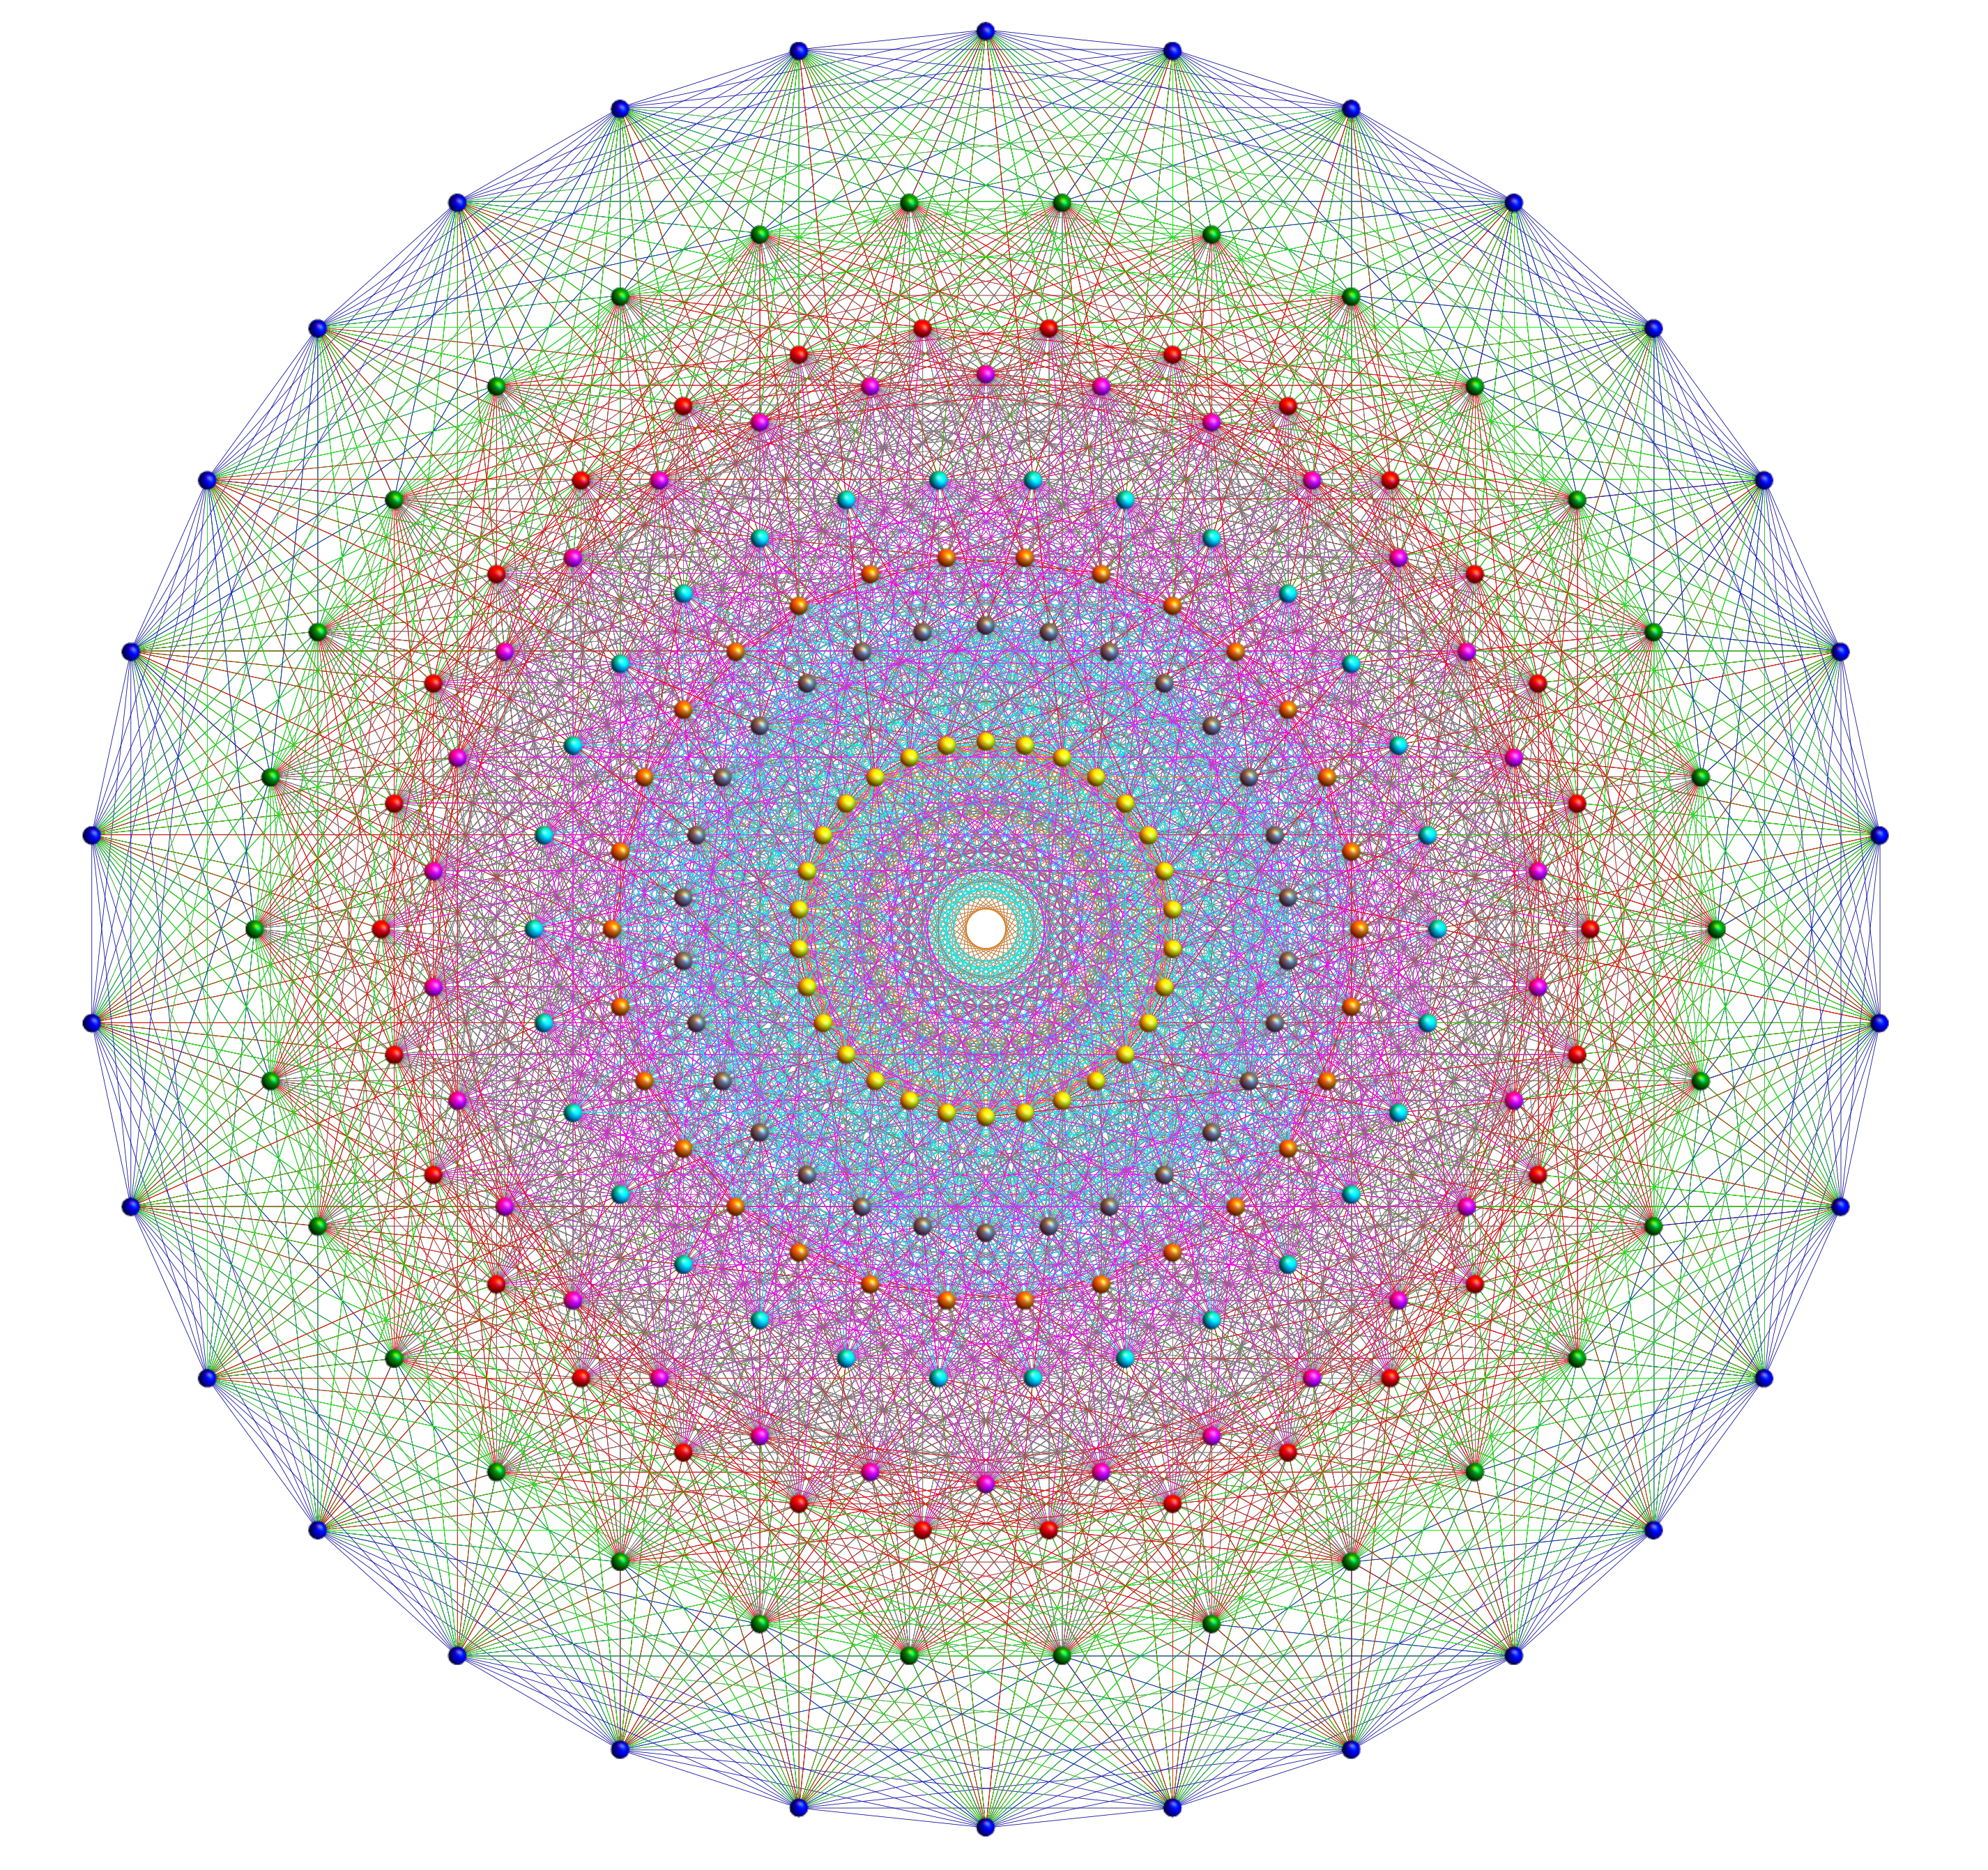
\includegraphics[width=.25\columnwidth]{front.png}
\end{figure}

\newpage
\tableofcontents 
\newpage

\section{Geometria proiettiva}
\subsection{Spazi proiettivi}
\begin{definizione}
	[Spazio proiettivo]
	Sia $V$ uno spazio vettoriale su un campo $\mathbb{K}$.
	Lo spazio proiettivo associato a $V$ \`e:
	\[
		\mathbb{P}(V) := \faktor{V\setminus\left\{ 0 \right\} }{\mathrm{\sim} }
	\] 
	con $v \sim w \iff \exists \lambda \in \mathbb{K}\setminus\left\{ 0 \right\} $ tale che $w = \lambda v$.
\end{definizione}
\noindent La relazione di equivalenza collassa tutti i vettori sulla stessa retta ad un unico elemento.
La mappa 
\[
\begin{array}
	{c c c}
	\mathbb{P}(V) & \longrightarrow & V \\
	\left[ v \right]  & \longmapsto & \operatorname{Span} (v)
\end{array}
\] 
\`e una biezione che associa ad ogni classe di equivalenza nel proiettivo il relativo span di un rappresentante in $V$ e, viceversa, ogni span di un elemento di $V$ \`e univocamente associato ad un elemento di $\mathbb{P}(V)$.
\begin{esempio}
	Si ha $\mathbb{P}(\left\{ 0 \right\} ) = \varnothing / \mathrm{\sim} = \varnothing $, mentre, dato $v \neq 0$ in $V$:
	\[
		\mathbb{P}(\operatorname{Span} (v)) = \faktor{\operatorname{Span} (v) \setminus\left\{ 0 \right\} }{\mathrm{\sim} } = \left\{ [v] \right\} 
	\] 
\end{esempio}
\begin{definizione}
	[Dimensione]
	La dimensione di uno spazio proiettivo \`e definita come:
	\[
	\dim _{\mathbb{K}} \mathbb{P}(V) := \dim _{\mathbb{K}} V - 1
	\] 
\end{definizione}
\noindent Di seguito, alcuni termini comunemente usati:
\begin{itemize}
	\item \textbf{punto proiettivo:} spazio proiettivo di dimensione $0$;
	\item \textbf{retta proiettiva:} spazio proiettivo di dimensione $1$;
	\item \textbf{piano proiettivo:} spazio proiettivo di dimensione $2$.
\end{itemize}
Infine, per \textbf{spazio proiettivo standard} si intende $\mathbb{P}(\mathbb{K}^{n+1} ) = \mathbb{P}^n(\mathbb{K}) = \mathbb{K}\mathbb{P}^n$.
\subsection{Trasformazioni proiettive}

\begin{definizione}
	[Trasformazione proiettiva]
	Una mappa $f : \mathbb{P}(V) \to \mathbb{P}(W)$ \`e una trasformazione proiettiva se esiste $\varphi : V \to  W	$ applicazione lineare tale che
	\[
		f([v]) = [\varphi (v)]
	\] 
	e si dice che $f$ \`e indotta da $\varphi $.
	In questo caso, si scriver\`a $f= [\varphi ]$.
\end{definizione}
\begin{prop}
	Se $f = [\varphi ]$ \`e una trasformazione proiettiva, allora $\varphi $ \`e iniettiva.
\end{prop}
\begin{proof}
	Per assurdo, se $\operatorname{Ker} \varphi \neq \left\{ 0 \right\} $, allora si troverebbe $v \in V$ tale che
	\[
		f([v]) = [\varphi (v)] = [0]
	\] 
	ma $[0] \not \in \mathbb{P}(W)$, quindi $f$ non sarebbe ben definita.
\end{proof}
\begin{prop}
Ogni trasformazione proiettiva \`e iniettiva.
\end{prop}
\begin{proof}
Sia $f : \mathbb{P}(V) \to \mathbb{P}(W)$ proiettiva indotta da $\varphi : V\to W$; allora 
\[
	[v] \xmapsto{\ f\ } [\varphi (v)] = [\varphi (w)] \iff \varphi (v) = \lambda \varphi (w) = \varphi (\lambda w)
\] 
Applicando la proposizione precedente, quindi, due elementi nell'immagine di $f$ coincidono se e solo se $v = \lambda w$, cio\`e se e solo se $[v]=[w]$.
\end{proof}
\begin{prop}
	Ogni applicazione lineare iniettiva $\varphi  : V \to  W$ induce una trasformazione proiettiva $f : \mathbb{P}(V) \to \mathbb{P}(W)$ tramite la mappa $[v] \longmapsto [\varphi (v)]$.
\end{prop}
\begin{proof}
	Si nota che, essendo $\varphi $ iniettiva, $[0] \not \in \mathbb{P}(W)$.
	Inoltre, se $[v] = [v']$ in $\mathbb{P}(V)$, cio\`e $v'= \lambda v$, allora $\varphi (v') = \varphi (\lambda v) = \lambda \varphi (v)$, per cui $[\varphi (v')] = [\varphi (v)]$.
\end{proof}
\begin{osservazione}
La mappa identit\`a $\operatorname{Id} _{\mathbb{P}(V)} $ \`e proiettiva ed \`e indotta da $\operatorname{Id} _V$.
\end{osservazione}
\begin{prop}
Date $f : \mathbb{P}(V) \to \mathbb{P}(W)$ e $g:\mathbb{P}(W) \to \mathbb{P}(Z)$, allora $g\circ f : \mathbb{P}(V) \to \mathbb{P}(Z)$ \`e proiettiva.
\end{prop}
Siano $f = [\varphi ]$ e $g = [\psi ]$.
Si mostra che $\psi \circ \varphi $ induce $g\circ f$; infatti:
\[
	[\psi \circ \varphi (v)] = g\big([\varphi (v)]\big) = g \circ f ([v])
\] 
\begin{definizione}
	[Isomorfismo proiettivo]
	Data $f$ proiettiva, questa \`e un isomorfismo proiettivo se \`e suriettiva.
\end{definizione}
\begin{teorema}
	[Caratterizzazione degli isomorfismi]
	Sia $f : \mathbb{P}(V) \to \mathbb{P}(W)$ proiettiva.
	Le seguenti affermazioni sono equivalenti:
	\begin{enumerate}[(a).]
		\item $f$ suriettiva;
		\item $f$ biettiva;
		\item $\dim \mathbb{P}(V) = \dim \mathbb{P}(W)$;
		\item $f$ invertibile e $f^{-1}:\mathbb{P}(W) \to \mathbb{P}(V)$ proiettiva.
	\end{enumerate}
\end{teorema}
\begin{proof}
Evidentemente (a)$\iff$(b), visto che ogni $f$ proiettiva \`e iniettiva.

Si ha (b)$\Rightarrow $(c) perch\'e, se $f = [\varphi ]$, allora $f$ biettiva implica $\varphi : V \to W$ isomorfismo lineare, per cui $\dim V = \dim W$, da cui la tesi.
Infatti, \`e immediato verificare che $f$ suriettiva $\Rightarrow \varphi $ suriettiva; se cos\`i non fosse, visto che se esiste $v \in V : \varphi (v) = w \implies \lambda w \in \operatorname{Im} \varphi $ perch\'e $\lambda v \xmapsto{\ \varphi \ } \lambda \varphi (v)=\lambda w, \ \forall \lambda \in \mathbb{K}$, allora un elemento non raggiunto da $\varphi $ corrisponde ad un intero sottospazio di dimensione $1$ non raggiunto in $W$, cio\`e ad un elemento non raggiunto da $f$ in $\mathbb{P}(W)$, che \`e assurdo perch\'e $f$ suriettiva.

Si ha (c)$\Rightarrow $(d) perch\'e $\dim \mathbb{P}(V) = \dim \mathbb{P}(W) \Rightarrow \dim V = \dim W$, quindi $\varphi $ \`e invertibile e, quindi, esiste un'applicazione lineare $\varphi ^{-1}$ che induce $f^{-1}$:
\[
	f^{-1}\circ f ([v]) = [\varphi ^{-1}\circ \varphi (v)] = [v]
\] 
ed \`e analogo per $f \circ f^{-1}$.
Quindi $f^{-1}=[\varphi ^{-1}]$ ed \`e proiettiva perch\'e $\varphi ^{-1}$ \`e iniettiva per costruzione.

Infine, (d)$\Rightarrow $(a) perch\'e $f$ invertibile implica $\varphi $ invertibile, quindi $\varphi $ suriettiva, quindi $f$ suriettiva.
\end{proof}
\begin{definizione}
	[Proiettivit\`a]
	Una trasformazione proiettiva $f : \mathbb{P}(V) \to \mathbb{P}(V)$ \`e detta proiettivit\`a.
	L'insieme delle proiettivit\`a di $\mathbb{P}(V)$ si indica con $\mathbb{P}\mathrm{GL} (V)$.
\end{definizione}
\begin{osservazione}
Ogni proiettivit\`a \`e un isomorfismo proiettivo per il teorema appena dimostrato ($\dim \mathbb{P}(V) = \dim \mathbb{P}(V)$).
Inoltre, $\big(\mathbb{P}\mathrm{GL} (V) , \circ\big)$ \`e un gruppo.
\end{osservazione}
\begin{osservazione}
	[Punti fissi]
	Sia $f=[\varphi ]$ una proiettivit\`a. 
	Assumendo che $[v]$ sia un punto fisso per $f$:
	\[
		[v]=f([v])=[\varphi (v)] \iff \varphi (v) = \lambda v
	\] 
	cio\`e $[v]$ \`e un punto fisso se e solo se $v$ \`e un autovettore di $\varphi $.
\end{osservazione}
\subsection{Sottospazi proiettivi}

\newpage
\section{Topologia generale}



\subsection{Spazi metrici}
\begin{definizione}
	[Spazio metrico]
Sia $X$ un insieme non vuoto; allora $X$ si dice spazio metrico se pu\`o essere equipaggiato con una \textit{distanza}, ossia una funzione $d : X \times X \to \mathbb{R}$ tale che:
\begin{itemize}
	\item $d(x,x') \ge  0 $ e $d(x,x') = 0 \iff x=x'$;
	\item $d(x,x') = d(x',x)$;
	\item $d(x,x'') \le  d(x,x') + d(x',x'')$.
\end{itemize}
\end{definizione}
\noindent Dato uno spazio metrico $(X,d_X)$ e un insieme $Y \subset  X$, si pu\`o definire un sottospazio di $(X,d_X)$ restringendo la distanza al solo $Y$:
\[
d_Y (y,y') := d_X(y,y'), \ \forall y,y' \in Y
\] 
Quindi $(Y,d_Y)$ \`e a sua volta uno spazio metrico, sottospazio di $(X,d_X)$, il quale \`e detto \textit{spazio ambiente} di $Y$.
In uno spazio metrico $(X,d)$, si pu\`o definire un \textit{disco aperto} di raggio $r$ e centro $x$ come
\[
B_r(x) := \left\{ x' \in X  \mid d(x,x') < r \right\} 
\] 
\begin{definizione}
	[Insieme aperto]
	Sia $(X,d)$ uno spazio metrico. Un suo sottoinsieme si dice aperto se \`e generato dall'unione di dischi aperti.
	
	Equivalentemente, un insieme $\forall \subseteq X$ si dice aperto rispetto alla metrica $d$ se $\forall x \in A, \ \exists \varepsilon >0 $ tale che $B_\varepsilon (x) \subseteq A$.
\end{definizione}
\begin{lemma}
	Le palle aperte sono insiemi aperti relativamente alla metrica che le definisce.
\end{lemma}
	\begin{proof}
		Sia $(X,d)$ uno spazio metrico e $x_0 \in X$; si dimostra che la palla $B_r(x_0) = \left\{ x \in X  \mid d(x_0,x) < r \right\} $ \`e aperto rispetto a $d$.
		Si nota che, $\forall x \in B_r(x_0)$, \`e possibile definire $\delta = r - d(x,x_0)$ tale che $B_\delta (x) \subseteq B_r(x_0)$; infatti tutti i punti di $B_\delta (x)$ sono a distanza minore di $\varepsilon $ da $x$, quindi, per disuguaglianza triangolare:
		\[
			d(x_0,y) \le d(x_0,x) + \underbracket{d(x,y)}_{< \delta }  < r, \ \forall y \in B_\delta (x)
		\] 
		per definizione di $\delta $.
	\end{proof}
\noindent Nello stesso spazio metrico, \`e possibile definire la distanza tra un punto $x \in X$ con un sottoinsieme $A \subseteq X$ come:
\begin{equation}
	d_A(x) = \inf \left\{ d(x,a)  \mid a \in A \right\}   
\end{equation}
\subsubsection{Continuit\`a in spazi metrici}
Una funzione $f:\mathbb{R}\to \mathbb{R}$ si dice continua in $x \in \mathbb{R}$ se $\forall \varepsilon , \ \exists \delta (\varepsilon )$ tale che:
\[
\lvert f(x) - f(x') \rvert < \varepsilon, \ \forall \lvert x-x' \rvert < \delta (\varepsilon )
\] 
\`E possibile generalizzare la definizione a spazi metrici usando la metrica definita su di essi.
\begin{definizione}
	[Continuit\`a in spazi metrici]
Sia $f : X\to Y$ un'applicazione, con $(X,d_X) , \ (Y,d_Y)$ spazi metrici. Si dice che $f$ \`e continua in $x \in X$ se $\forall \varepsilon , \ \exists \delta (\epsilon )$ tale che:
\begin{equation}
	d_Y \big(f(x), f(x')\big) < \varepsilon , \ \forall d_X(x,x')< \delta (\varepsilon )
\end{equation}
Questo si esprime equivalentemente come:
\[
\forall \varepsilon >0, \ \exists \delta > 0 \text{ t.c. } f(B_{d_X} (x,\delta )) \subseteq B_{d_Y} (f(x),\varepsilon )
\] 

\end{definizione}
\noindent Usando la nozione di insieme aperto, \`e possibile generalizzare ulteriormente la definizione di continuit\`a al solo concetto di apertura di un insieme.
\begin{teorema}
Un'applicazione $f:X\to Y$ \`e continua $\iff\forall A \subset  Y$ aperto, l'insieme $f^{-1}(A)  $ \`e aperto.
\end{teorema}
\begin{proof}
Si dimostrano le due implicazioni.	
\begin{itemize}
	\item $(\Rightarrow )$ Si assume che $f$ sia continua. Si prende $f(x) \in A$, con $A\subset Y$ aperto, per qualche $x \in f^{-1} (A)$. Essendo $A$ aperto $\Rightarrow \exists \varepsilon >0 : B_\varepsilon \big(f(x)\big)\subset A$; allo stesso tempo, per continuit\`a di $f$, dato $\varepsilon $ scelto prima, deve esistere $\delta (\varepsilon )$ tale che
		\[
		f\big(B_{\delta (\varepsilon )}(x)\big) \subset B_\varepsilon \big(f(x)\big)
		\] 
	quindi $B_{\delta (\varepsilon )} (x) \subset f^{-1} (A)$. Valendo $\forall x \in f^{-1} (A)\Rightarrow f^{-1} (A)$ \`e aperto perch\'e per ogni suo elemento, esiste una palla tutta contenuta al suo interno.
\item $(\Leftarrow)$ Si assume che $\forall A \subset Y$ aperto, la funzione $f$ sia tale che l'insieme $f^{-1} (A)$ \`e aperto. Per $f(x) \in Y$, esiste $B_\varepsilon \big(f(x)\big) \subset Y$; essendo questo aperto, deve essere aperto anche $f^{-1} \big[B_\varepsilon \big(f(x)\big) \big]$. 
	Dunque, dato $x \in f^{-1} \big[B_\varepsilon \big(f(x)\big) \big] $, $\exists \delta (\varepsilon ) : B_{\delta (\varepsilon )} (x) \subset f^{-1} \big[B_\varepsilon \big(f(x)\big) \big]$, quindi vuol dire che $f\big(B_{\delta (\varepsilon )} (x)\big)\subset B_\varepsilon \big(f(x)\big)$, ossia:
	\[
	d_Y\big(f(x), f(x')\big) < \varepsilon , \ \forall d_X (x,x') < \delta (\varepsilon )
	\] 
Valendo $\forall x \in X$, allora $f$ \`e continua.
\end{itemize}
\end{proof}
\noindent Questo permette di parlare di continuit\`a di applicazioni in insiemi su cui non \`e definita una distanza, ma solo i sottoinsiemi aperti.

Negli spazi metrici, \`e possibile caratterizzare delle mappe che preservano le distanze; queste sono note come \textit{immersioni isometriche}.
\begin{definizione}
	[Immersione isometrica]
	Sia $f:X\to Y$ una mappa tra spazi metrici; questa \`e detta immersione isometrica se
	\[
	d_Y(f(x),f(y)) = d_X(x,y)
	\] 
\end{definizione}
\noindent Un'immersione isometrica deve necessariamente essere iniettiva:
\[
f(x) = f(y) \implies d_Y(f(x),f(y))= 0 = d_X(x,y) \iff x=  y 
\] 
Inoltre, la composizione di due immersioni isometriche \`e ancora un'immersione isometrica e l'identit\`a ne \`e un esempio.
\begin{definizione}
	[Isometria]
	Sia $f:X\to Y$ un'immersione isometrica; allora se $f$ \`e suriettiva, quindi biettiva, \`e detta \textit{isometria}.
\end{definizione}
\noindent Le isometrie formano un gruppo con l'operazione di composizione, che si indica con $\mathrm{Isom} (X)$.
\begin{definizione}
	[Omeomorfismo]
	Dati $X,Y$ spazi metrici, un'applicazione biettiva $f:X\to Y$ \`e un \textit{omeomorfismo} se la sua inversa e $f$ stessa sono continue.
\end{definizione}
\noindent Ne segue che ogni isometria \`e un omeomorfismo, ma non \`e vero il viceversa. Per esempio, definendo $e^x : \mathbb{R} \to (0,+\infty)$, questa ha un'inversa continua $\log(x) : (0,+\infty) \to \mathbb{R}$, quindi \`e un omeomorfismo, ma non \`e un'isometria perch\'e manda $(-\infty,0]$ in $(0,1]$.
Anche gli omemorfismi definiscono una \textbf{relazione di equivalenza} tra spazi metrici.
\begin{definizione}
	[Mappa lipschitziana]
	Siano $(X,d_X)$ e $(Y,d_Y)$ due spazi metrici e sia $f : X \to Y$ una mappa; si dice che $f$ \`e \textit{lipschitizana} se 
	\[
	d_Y(f(p),f(q)) \le kd_X(p,q) ,\ \forall p,q \in X
	\] 
\end{definizione}
\begin{prop}
	Se $f:X\to Y$ \`e lipschitizana, allora \`e continua.
\end{prop}
	\begin{proof}
		Sia $f$ una funzione $k$-lipschitziana; si fissa $\varepsilon > 0 $ e si prende $\delta = \varepsilon / k$, per cui $\forall x' \in X$ tale che $d_X (x,x') < \delta $, si ha
		\[
		d_Y(f(x),f(x')) \le k d_X(x,x') < k \frac{ \varepsilon}{k}  = \varepsilon 
		\] 
		
	\end{proof}
\subsection{Spazi topologici}
Allo scopo di giustificare la definizione e lo studio di spazi topologici, si considera il seguente risultato.
\begin{prop}
	Sia $(X,d)$ uno spazio metrico. Allora:
	\begin{enumerate}[(a).]
		\item $\varnothing$ e $X$ sono aperti;
		\item se $A,B$ sono aperti, allora $A\cap B$ \`e aperto;
		\item se $\left\{ A_i \right\} _{i\in I} $ \`e una famiglia di aperti, allora $\bigcup_{i \in I} A_i$ \`e aperto.
	\end{enumerate}
\end{prop}
	\begin{proof}
		Si divide la dimostrazione nei vari punti.
		\begin{enumerate}[(a).]
			\item $X$ \`e ovviamente aperto, mentre per l'insieme vuoto non ci sono punti per cui bisogna verificare la richiesta, quindi \`e aperto.
			\item Sia $x_0 \in A\cap B$; questo significa che ci sono due palle di raggi $\epsilon _1, \epsilon _2$ interamente contenute in $A$ e $B$ rispettivamente, visto che sono aperti.
				Prendendo $\epsilon = \min \left\{ \epsilon _1,\epsilon _2 \right\} $, si verifica immediatamente che $B_\epsilon (x) \subseteq A\cap B$, visto che \`e interamente contenuta sia in $A$ che $B$.
			\item Evidentemente $\exists j \in I : x_0 \in A_j \implies \exists \epsilon : B_\epsilon (x_0) \subseteq A_j \subseteq \bigcup_{i \in I} A_i$.
		\end{enumerate}
	\end{proof}
\noindent Si nota che l'intersezione arbitraria di aperit pu\`o non risultare aperta, come nel caso della famiglia $B_{1 / n} (0)$ in $\mathbb{R}$.

Dalla precedente proposizione, \`e possibile giustificare la seguente definizione di topologia.
\begin{definizione}
	[Topologia e spazio topologico]
	Sia $X$ un insieme non-vuoto. Una \textit{topologia} su $X$ \`e una famiglia non-vuota $\tau \subseteq \mathcal{P} (x)$, chiamati \textit{insiemi aperti della topologia}. Questi soddisfano le seguenti condizioni:
	\begin{itemize}
		\item $\varnothing, \ X$ sono aperti;
		\item l'unione di una qualsiasi famiglia di insiemi aperti \`e un insieme aperto;
		\item l'intersezione di due insiemi aperti \`e un aperto.
	\end{itemize}
	Allora si definisce \textit{spazio topologico} la coppia $(X,\tau )$, dove $X$ \`e detto \textit{supporto} dello spazio topologico e i suoi elementi sono i \textit{punti} dello spazio.
\end{definizione}





\end{document}
